\documentclass[12pt]{article}
\usepackage{amsmath}
\usepackage{amsthm}
\usepackage{amssymb}
\usepackage{bm}
\usepackage[round]{natbib}
\usepackage{bm}
\newcommand{\Le}{\left(}
\newcommand{\Ri}{\right)}
\newcommand{\N}{\mathbb{N}}
\newcommand\independent{\protect\mathpalette{\protect\independenT}{\perp}}
\def\independenT#1#2{\mathrel{\rlap{$#1#2$}\mkern2mu{#1#2}}}
\newtheorem{theorem}{Theorem}
\newtheorem{definition}{Definition}
\newtheorem{corollary}{Corollary}
\newtheorem{lemma}{Lemma}

\date{}
\title{Supplementary Material for the article \textit{Quotient Normalized Maximum Likelihood Criterion for Learning Bayesian Network Structures} }
\begin{document}
\maketitle

\appendix
\section{Regularity proof}

\subsection{Preliminaries}
We start by recalling the definition of regularity \citep{Suzuki2017}:

\begin{definition}
Assume $H_N(X \mid Y') \leq H_N(X \mid Y)$, where $Y' \subset Y.$ We say that the scoring function $Q_N(\cdot \mid \cdot)$ is regular if $Q_n(X \mid Y') \geq Q_N(X \mid Y)$.
\end{definition}
In the definition, $N$ denotes the sample size, $X$ is some random variable, $Y$ denotes the proposed parent set for $X$, and $H_N(X \mid Y)$ refers to the empirical conditional entropy based on $N$ samples of variables $X$ and $Y$.

Let $X$ be a categorical random variable with $r$ possible values. Let $U$ denote a possible parent set with $q$ different combinations of values for the variables, and $V$ a parent set with $m$ different configurations. Assume that we have observed $N$ samples of $(X,U,V)$ (denoted by $x_N,u_N$ and $v_N$) and $H_N(X \mid U) \leq H_N(X \mid U \cup V)$ holds.

Recall the definition of the qNML score:
\begin{align*}
Q^{qnml}_N(X\mid U) &= \log P(x_n \mid \hat{\theta}_{X\mid U} \ ) - \Le reg(N,rq) - reg(N,q) \Ri \\
&= \log P(x_N \mid \hat{\theta}_{X\mid U} \ ) - \log \frac{C(N,rq)}{C(N,q)},
\end{align*}where $C(N,r)$ is the normalizing constant the of the NML distribution for a categorical variable with $r$ possible values and sample size $N$ and $ \hat{\theta}_{X\mid U}$ denotes the maximum likelihood parameters of the conditional distribution of $X$ given $U$ which are computed from the data $(x_N,u_N)$. 


In order to prove the regularity, we need the following three lemmas:
\begin{lemma}\label{Cpolynom} We can write $C(N,k)$ as a polynomial of $k$, formally
$$
C(N,k) = \sum_{j=1}^N a_j k^j,
$$where $a_j > 0$. 
\end{lemma}
\begin{lemma}\label{MLterms}
Assume $H_N(X \mid Y') \leq H_N(X \mid Y)$, where $Y' \subset Y$. Now $\log P(x_N \mid \hat{\theta}_{X\mid Y} \ ) = \log P(x_N \mid \hat{\theta}_{X\mid Y'} \ )$.
\end{lemma}
\begin{lemma}\label{increasing}
Let $r \in \N, r \geq 2$.  The function $k \mapsto \frac{C(N,rk)}{C(N,k)}$ is increasing for every $k \geq 2$.
\end{lemma}
\noindent We present the proofs of these lemmas in Section \ref{lemmaproofs}.  

\subsection{The main proof}
\begin{theorem}
qNML score is regular.
\end{theorem}
\begin{proof}
We want to show that
$$
Q^{qnml}_N(X\mid U) \geq Q^{qnml}_N(X \mid U \cup V).
$$assuming $H_N(X \mid U) \leq H_N(X \mid U \cup V)$. Using the entropy assumption and Lemma \ref{MLterms} implies that the maximized likelihood terms are equal. In order to prove the claim, it suffices to study the penalty terms, and we want to show that
\begin{align*}
- \Le reg(N,rq) - reg(N,q) \Ri \ &\geq \  -\Le reg(N,rqm) - reg(N,qm) \Ri \\
\log \frac{C(N,rq)}{C(N,q)} \ &\leq \log \frac{C(N,rqm)}{C(N,qm)}.
\end{align*}This holds, since logarithm is an increasing function, and $q \leq qm$, so we can apply Lemma \ref{increasing} to conclude the proof. 


\end{proof}


\subsection{Proofs of lemmas}\label{lemmaproofs}
%We want to show that
%$$
%\quad  Q^{qnml}_N(X\mid U) \geq Q^{qnml}_N(X \mid U \cup V)
%$$which, by using the definition of qNML, is equivalent to 
%\begin{equation}\label{statement}
%\log P(X \mid )
%\end{equation}
%The assumption about entropy implies that the maximized likelihood terms of the qnml-score are equal. 
\setcounter{lemma}{0}
\begin{lemma} $C(N,k)$ can be written as a polynomial of $k$, formally
$$
C(N,k) = \sum_{j=1}^N a_j k^j,
$$where $a_j > 0$. 
\end{lemma}
\begin{proof} \cite{cosco.itsl08} derive the following representation for the normalizing constant
\begin{align*}  
C(N,k) = \sum_{l=0}^{N-1}\frac{(N-1)^{\underline{l}}k^{\overline{l + 1}}}{N^{l+1} \ l!} ,
\end{align*}where $x^{\underline{l}}$ and $x^{\overline{l}}$ denote falling and rising factorials, respectively. 

We utilize the fact that the rising factorial can be represented as polynomial using unsigned Stirling numbers of the first kind (see \cite{Adamchik1997}, for instance)
\begin{align*}
C(N,k) &=  \sum_{l=0}^{N-1}\frac{(N-1)^{\underline{l}}k^{\overline{l + 1}}}{N^{l+1} \ l!} \\
&= \sum_{l=0}^{N-1} b_l \ k^{\overline{l+1}} \\
&= \sum_{l=0}^{N-1} b_l \Le \sum_{j=1}^{l+1}|s(l + 1,j)| \ k^j \Ri \\
&= \sum_{l=0}^{N-1} \Le \sum_{j=1}^{N}b_l \ |s(l + 1,j)| \ k^j \Ri \\
&= \sum_{j=1}^{N} \Le \sum_{l=0}^{N-1} b_l \ |s(l + 1,j)| \ k^j \Ri \\
&= \sum_{j=1}^{N} \Le \sum_{l=0}^{N-1} b_l \ |s(l + 1,j)| \Ri k^j \\
&= \sum_{j=1}^{N} a_j  k^j,
\end{align*}where $s(i,j)$ denotes the (signed) Stirling number of the first kind and
$$
a_j = \Le \sum_{l=0}^{N-1} \frac{(N-1)^{\underline{l}}}{N^{l+1}l!} \ |s(l + 1,j)| \Ri,
$$ $a_j > 0$ for all $j$. On the second row, we denoted $b_l = (N-1)^{\underline{l}}/(N^{l+1} l!)$. On the row 4, we used the property of Stirling numbers: $s(i,j) = 0$ for all $j > i$. 
\end{proof}
\begin{lemma}
Assume $H_N(X \mid Y') \leq H_N(X \mid Y)$, where $Y' \subset Y$. Now $\log P(x_N \mid \hat{\theta}_{X\mid Y} \ ) = \log P(x_N \mid \hat{\theta}_{X\mid Y'})$.
\end{lemma}
\begin{proof}
We can write the logarithm of the maximized likelihood, \\ $\log P(x_N \mid \hat{\theta}_{X\mid Y} \ )$, as follows \citep{KOLLER}
\begin{align*}
\log P(x_N \mid \hat{\theta}_{X\mid Y} \ ) & = -N \Le H_N(X) - I_N(X;Y) \Ri \\
&= -N \  H_N(X\mid Y),
\end{align*}where $I_N(\cdot;\cdot)$ is the empirical mutual information. This implies that the assumption
$$
H_N(X \mid Y') \leq H_N(X \mid Y)
$$ is equivalent to
$$
\log P(x_N \mid \hat{\theta}_{X\mid Y} \ ) \geq \log P(x_N \mid \hat{\theta}_{X\mid Y'} \ ) .
$$Actually we must have the equality holding in the above expression, since
$$
H_N(X \mid Y') < H_N(X \mid Y)
$$ would imply that
$$
I_N(X ; Z \mid Y ) < 0,
$$where $Z = Y \setminus Y'$, which is impossible.
\end{proof}
\begin{lemma}
Let $r \in \N, r \geq 2$.  The function $k \mapsto \frac{C(N,rk)}{C(N,k)}$ is increasing for every $k \geq 2$.
\end{lemma}

\begin{proof}
Lemma \ref{Cpolynom} lets us to write
\begin{equation}\label{C1}
C(N,k) = \sum_{j=1}^{N} a_j k^j
\end{equation}and, similarly,
\begin{equation}\label{C2}
C(N,rk) = \sum_{j=1}^{N} a_j  r^jk^j.
\end{equation}

From this, it it easy see that the derivative of the quotient, \\ $d/dk (C(N,rk)/C(N,k))$, will be a ratio of two polynomials of $k$. Our goal is to show that the polynomial in the numerator has positive coefficients, which will guarantee the positivity of derivative for every $k > 0$, and thus imply that the original function is increasing (polynomial in the denominator is squared and non-zero for $k > 0$, so it can be ignored).  

Derivatives of (\ref{C1}) and (\ref{C2}) are obtained easily:
\begin{align*}
\frac{d}{dk}C(N,k) &= \sum_{j=1}^{N}ja_jk^{j-1} \\
&= \sum_{j=0}^{N-1}(j+1) a_{j+1}k^{j}
\end{align*}and
\begin{align*}
\frac{d}{dk}C(N,rk) &= \sum_{j=1}^{N}ja_jr^jk^{j-1} \\
&= \sum_{j=0}^{N-1}(j+1)a_{j+1}r^{j+1}k^{j}. 
\end{align*}Consider next the products found in the derivative of the quotient. We obtain
\begin{align*}
\Le\frac{d}{dk}C(N,rk)\Ri C(N,k) &= \Le \sum_{j=0}^{N-1}(j+1)a_{j+1}r^{j+1}k^{j} \Ri \Le \sum_{l=1}^{N} a_l  k^l \Ri \\
&= \sum_{i = 1}^{2N-1} \Le \sum_{j+l = i} (j+1)a_{j+1}r^{j+1}a_l  \Ri k^i
\end{align*}and
%\begin{align*}
%\Le\frac{d}{dk}C(n,k)\Ri C(n,rk) &= \Le \sum_{j=0}^{n-1}(j+1)a_{j+1}k^{j} \Ri \Le %\sum_{l=1}^{n} a_l  r^lk^l  \Ri \\
%&= \sum_{i = 1}^{2n-1} \Le \sum_{m=0}^i (m+1)a_{m+1}a_{i-m}r^{i-m}   \Ri k^i
%\end{align*}
\begin{align*}
\Le\frac{d}{dk}C(N,k)\Ri C(N,rk) &= \Le \sum_{j=0}^{N-1}(j+1)a_{j+1}k^{j} \Ri \Le \sum_{l=1}^{N} a_l  r^lk^l  \Ri \\
&= \sum_{i = 1}^{2N-1} \Le \sum_{j+l = i}(j+1)a_{j+1}a_l  r^l   \Ri k^i.
\end{align*}
Subtracting these two expression yields
\begin{align*}
&\Le\frac{d}{dk}C(N,rk)\Ri C(N,k)-\Le\frac{d}{dk}C(N,k)\Ri C(N,rk) \\&= \sum_{i = 1}^{2N-1} \Le \sum_{j+l = i} (j+1)a_{j+1}r^{j+1}a_l  \Ri k^i - \sum_{i = 1}^{2N-1} \Le \sum_{j+l = i}(j+1)a_{j+1}a_l  r^l   \Ri k^i \\
&= \sum_{i = 1}^{2N-1} \Le \sum_{j+l = i}(j+1)a_{j+1}a_l  (r^{j+1}- r^l)   \Ri k^i
\end{align*}which is the polynomial in the numerator of the derivative of $C(N,rk)/C(N,k)$.
Next, we study the coefficient of $k^i$, if $i \leq N$
\begin{align*}
\sum_{j+l = i}(j+1)a_{j+1}a_l  (r^{j+1}- r^l) &= \sum_{l=1}^{i}(i-l+1)a_{i-l+1}a_l  (r^{i-l+1}- r^l) \\
& = \sum_{l=1}^{i}(i-l+1)c_l \\
&= \sum_{k =1}^{\lfloor i / 2 \rfloor}(i-k+1)c_k + (i-(i-k + 1)+1)c_{i-k+1} \\
&=  \sum_{k =1}^{\lfloor i / 2 \rfloor}(i-k+1)c_k + kc_{i-k+1} \\
&=  \sum_{k =1}^{\lfloor i / 2 \rfloor}(i-k+1)c_k - kc_{k} \\
&= \sum_{k =1}^{\lfloor i / 2 \rfloor}(i-2k+1)c_k.
\end{align*} On the first row, we re-wrote sum using only one running index. On the second row we denoted $c_l =a_{i-l+1}a_l  (r^{i-l+1}- r^l)$. On the third row, we re-arranged the sum so that we are summing over pairs of terms of the original sum: the first and the last term, the second and the second to last, and so on.  This resulting sum has $\lfloor i / 2 \rfloor$ terms. We have to use the floor-function since if $i$ is odd, there exists an index $l'$ in the original sum such that $r^{i-l'+1}-r^{l'} = 0$. On the fifth row, we make use of the identity $c_k = -c_{i-k+1}$ which is straightforward to verify. From the last row, we can observe that every term of the sum is positive since $i-2k+1$ and $r^{i-k+1}- r^k$ are both positive if $k \leq (i+1)/2$ which holds since $k$ ranges from $1$ to $\lfloor i / 2 \rfloor$.

Let us now consider the situation where $n < i \leq 2N-1$. We start with the special case where $i = 2N-1$. Then, we have only one term in the sum
\begin{align*}
\sum_{j+l = i}(j+1)a_{j+1}a_l  (r^{j+1}- r^l) &= \sum_{l=N}^{N}(2N-1-l+1)a_{2N-1-l+1}a_l  (r^{2N-1-l+1}- r^l) \\
&= Na_{N}a_N  (r^{N}- r^N) \\
& = 0.
\end{align*}Now, let $N < i < 2N-1$, we follow a similar procedure as before to manipulate the sum
\begin{align*}
\sum_{j+l = i}(j+1)a_{j+1}a_l  (r^{j+1}- r^l) &= \sum_{l=i-N + 1}^{N}(i-l+1)a_{i-l+1}a_l  (r^{i-l+1}- r^l) \\
& = \sum_{l=i-N + 1}^{N}(i-l+1)c_l \\
& = \sum_{k=1}^{2N-i}(N-k+1)c_{i-N+k} \\
& = \sum_{k=1}^{\lfloor N - i/2 \rfloor}(N-k+1)c_{i-N+k}\\
&+  (N-(2N-i-k+1)+1)c_{i-N+(2N-i-k+1)} \\
&= \sum_{k=1}^{\lfloor N - i/2 \rfloor}(N-k+1)c_{i-N+k} +  (i-N+k)c_{N-k+1} \\
&= \sum_{k=1}^{\lfloor N - i/2 \rfloor}(N-k+1)c_{i-N+k} -  (i-N+k)c_{i-N+k} \\
&= \sum_{k=1}^{\lfloor N - i/2 \rfloor}(N-k+1-(i-N+k))c_{i-N+k} \\
&= \sum_{k=1}^{\lfloor N - i/2 \rfloor}(2N-i-2k+1)c_{i-N+k}.
\end{align*}It is now easy to verify that $(2N-i-2k+1)$ and $c_{i-N+k}$ are positive if $k \leq N - (i-1)/2$ which holds since $k$ ranges from $1$ to $\lfloor N - i/2 \rfloor$. The floor function is again used when we sum over pairs of terms since if $i$ is odd there is zero-term. 
Since all the coefficients are non-negative and the $k \geq 2$, the derivative is positive. This implies that the original function is increasing.
\end{proof}
\newpage
\section{Regularity proof}

\subsection{Preliminaries}
We start by recalling the definition of regularity \citep{Suzuki2017}:

\begin{definition}
Assume $H_N(X \mid Y') \leq H_N(X \mid Y)$, where $Y' \subset Y.$ We say that the scoring function $Q_N(\cdot \mid \cdot)$ is regular if $Q_N(X \mid Y') \geq Q_N(X \mid Y)$.
\end{definition}
In the definition, $N$ denotes the sample size, $X$ is some random variable, $Y$ denotes the proposed parent set for $X$, and $H_N(X \mid Y)$ refers to the empirical conditional entropy based on $N$ samples of variables $X$ and $Y$.

Let $X$ be a categorical random variable with $r$ possible values. Let $U$ denote a possible parent set with $q$ different combinations of values for the variables, and $V$ a set with $m$ different configurations. Assume that we have observed $N$ samples of $(X,U,V)$ (denoted by $x_N,u_N$ and $v_N$) and $H_N(X \mid U) \leq H_N(X \mid U \cup V)$ holds.

Recall the definition of the qNML score:
\begin{align*}
Q^{qnml}_N(X\mid U) &= \log P(x_N \mid \hat{\theta}_{X\mid U} \ ) - \Le reg(N,rq) - reg(N,q) \Ri \\
&= \log P(x_N \mid \hat{\theta}_{X\mid U} \ ) - \log \frac{C(N,rq)}{C(N,q)},
\end{align*}where $C(N,r)$ is the normalizing constant the of the NML distribution for a categorical variable with $r$ possible values and sample size $N$ and $ \hat{\theta}_{X\mid U}$ denotes the maximum likelihood parameters of the conditional distribution of $X$ given $U$ which are computed from the data $(x_N,u_N)$. 


In order to prove the regularity, we need the following three lemmas:
\begin{lemma}\label{Cpolynom} We can write $C(N,k)$ as a polynomial of $k$, formally
$$
C(N,k) = \sum_{j=1}^N a_j k^j,
$$where $a_j > 0$. 
\end{lemma}
\begin{lemma}\label{MLterms}
Assume $H_N(X \mid Y') \leq H_N(X \mid Y)$, where $Y' \subset Y$. Now $\log P(x_N \mid \hat{\theta}_{X\mid Y} \ ) = \log P(x_N \mid \hat{\theta}_{X\mid Y'} \ )$.
\end{lemma}
\begin{lemma}\label{increasing}
Let $r \in \N, r \geq 2$.  The function $k \mapsto \frac{C(N,rk)}{C(N,k)}$ is increasing for every $k \geq 2$.
\end{lemma}
\noindent We present the proofs of these lemmas in Section \ref{lemmaproofs}.  

\subsection{The main proof}
\begin{theorem}
qNML score is regular.
\end{theorem}
\begin{proof}
We want to show that
$$
Q^{qnml}_N(X\mid U) \geq Q^{qnml}_N(X \mid U \cup V).
$$assuming $H_N(X \mid U) \leq H_N(X \mid U \cup V)$. Using the entropy assumption and Lemma \ref{MLterms} implies that the maximized likelihood terms are equal. In order to prove the claim, it suffices to study the penalty terms, and we want to show that
\begin{align*}
- \Le reg(N,rq) - reg(N,q) \Ri \ &\geq \  -\Le reg(N,rqm) - reg(N,qm) \Ri \\
\log \frac{C(N,rq)}{C(N,q)} \ &\leq \log \frac{C(N,rqm)}{C(N,qm)}.
\end{align*}This holds, since logarithm is an increasing function, and $q \leq qm$, so we can apply Lemma \ref{increasing} to conclude the proof. 


\end{proof}


\subsection{Proofs of lemmas}\label{lemmaproofs}
%We want to show that
%$$
%\quad  Q^{qnml}_N(X\mid U) \geq Q^{qnml}_N(X \mid U \cup V)
%$$which, by using the definition of qNML, is equivalent to 
%\begin{equation}\label{statement}
%\log P(X \mid )
%\end{equation}
%The assumption about entropy implies that the maximized likelihood terms of the qnml-score are equal. 
\setcounter{lemma}{0}
\begin{lemma} $C(N,k)$ can be written as a polynomial of $k$, formally
$$
C(N,k) = \sum_{j=1}^N a_j k^j,
$$where $a_j > 0$. 
\end{lemma}
\begin{proof} \cite{cosco.itsl08} derive the following representation for the normalizing constant
\begin{align*}  
C(N,k) = \sum_{l=0}^{N-1}\frac{(N-1)^{\underline{l}}k^{\overline{l + 1}}}{N^{l+1} \ l!} ,
\end{align*}where $x^{\underline{l}}$ and $x^{\overline{l}}$ denote falling and rising factorials, respectively. 

We utilize the fact that the rising factorial can be represented as polynomial using unsigned Stirling numbers of the first kind (see \cite{Adamchik1997}, for instance)
\begin{align*}
C(N,k) &=  \sum_{l=0}^{N-1}\frac{(N-1)^{\underline{l}}k^{\overline{l + 1}}}{N^{l+1} \ l!} \\
&= \sum_{l=0}^{N-1} b_l \ k^{\overline{l+1}} \\
&= \sum_{l=0}^{N-1} b_l \Le \sum_{j=1}^{l+1}|s(l + 1,j)| \ k^j \Ri \\
&= \sum_{l=0}^{N-1} \Le \sum_{j=1}^{N}b_l \ |s(l + 1,j)| \ k^j \Ri \\
&= \sum_{j=1}^{N} \Le \sum_{l=0}^{N-1} b_l \ |s(l + 1,j)| \ k^j \Ri \\
&= \sum_{j=1}^{N} \Le \sum_{l=0}^{N-1} b_l \ |s(l + 1,j)| \Ri k^j \\
&= \sum_{j=1}^{N} a_j  k^j,
\end{align*}where $s(i,j)$ denotes the (signed) Stirling number of the first kind and
$$
a_j = \Le \sum_{l=0}^{N-1} \frac{(N-1)^{\underline{l}}}{N^{l+1}l!} \ |s(l + 1,j)| \Ri,
$$ $a_j > 0$ for all $j$. On the second row, we denoted $b_l = (N-1)^{\underline{l}}/(N^{l+1} l!)$. On the row 4, we used the property of Stirling numbers: $s(i,j) = 0$ for all $j > i$. 
\end{proof}
\begin{lemma}
Assume $H_N(X \mid Y') \leq H_N(X \mid Y)$, where $Y' \subset Y$. Now $\log P(x_N \mid \hat{\theta}_{X\mid Y} \ ) = \log P(x_N \mid \hat{\theta}_{X\mid Y'})$.
\end{lemma}
\begin{proof}
We can write the logarithm of the maximized likelihood, \\ $\log P(x_N \mid \hat{\theta}_{X\mid Y} \ )$, as follows \citep{KOLLER}
\begin{align*}
\log P(x_N \mid \hat{\theta}_{X\mid Y} \ ) & = -N \Le H_N(X) - I_N(X;Y) \Ri \\
&= -N \  H_N(X\mid Y),
\end{align*}where $I_N(\cdot;\cdot)$ is the empirical mutual information. This implies that the assumption
$$
H_N(X \mid Y') \leq H_N(X \mid Y)
$$ is equivalent to
$$
\log P(x_N \mid \hat{\theta}_{X\mid Y} \ ) \leq \log P(x_N \mid \hat{\theta}_{X\mid Y'} \ ) .
$$Actually we must have the equality holding in the above expression, since
$$
H_N(X \mid Y') < H_N(X \mid Y)
$$ would imply that
$$
I_N(X ; Z \mid Y ) < 0,
$$where $Z = Y \setminus Y'$, which is impossible.
\end{proof}
\begin{lemma}
Let $r \in \N, r \geq 2$.  The function $k \mapsto \frac{C(N,rk)}{C(N,k)}$ is increasing for every $k \geq 2$.
\end{lemma}

\begin{proof}
Lemma \ref{Cpolynom} lets us to write
\begin{equation}\label{C1}
C(N,k) = \sum_{j=1}^{N} a_j k^j
\end{equation}and, similarly,
\begin{equation}\label{C2}
C(N,rk) = \sum_{j=1}^{N} a_j  r^jk^j.
\end{equation}

In the following, we assume that $k$ is a real number. From (\ref{C1}) and (\ref{C2}), it is easy see that the derivative of the quotient, $d/dk (C(N,rk)/C(N,k))$, will be a ratio of two polynomials of $k$. Our goal is to show that the polynomial in the numerator has positive coefficients, which will guarantee the positivity of derivative for every $k > 0$, and thus imply that the original function is increasing (polynomial in the denominator is squared and non-zero for $k > 0$, so it can be ignored).  

Derivatives of (\ref{C1}) and (\ref{C2}) are obtained easily:
\begin{align*}
\frac{d}{dk}C(N,k) &= \sum_{j=1}^{N}ja_jk^{j-1} \\
&= \sum_{j=0}^{N-1}(j+1) a_{j+1}k^{j}
\end{align*}and
\begin{align*}
\frac{d}{dk}C(N,rk) &= \sum_{j=1}^{N}ja_jr^jk^{j-1} \\
&= \sum_{j=0}^{N-1}(j+1)a_{j+1}r^{j+1}k^{j}. 
\end{align*}Consider next the products found in the derivative of the quotient. We obtain
\begin{align*}
\Le\frac{d}{dk}C(N,rk)\Ri C(N,k) &= \Le \sum_{j=0}^{N-1}(j+1)a_{j+1}r^{j+1}k^{j} \Ri \Le \sum_{l=1}^{N} a_l  k^l \Ri \\
&= \sum_{i = 1}^{2N-1} \Le \sum_{j+l = i} (j+1)a_{j+1}r^{j+1}a_l  \Ri k^i
\end{align*}and
%\begin{align*}
%\Le\frac{d}{dk}C(n,k)\Ri C(n,rk) &= \Le \sum_{j=0}^{n-1}(j+1)a_{j+1}k^{j} \Ri \Le %\sum_{l=1}^{n} a_l  r^lk^l  \Ri \\
%&= \sum_{i = 1}^{2n-1} \Le \sum_{m=0}^i (m+1)a_{m+1}a_{i-m}r^{i-m}   \Ri k^i
%\end{align*}
\begin{align*}
\Le\frac{d}{dk}C(N,k)\Ri C(N,rk) &= \Le \sum_{j=0}^{N-1}(j+1)a_{j+1}k^{j} \Ri \Le \sum_{l=1}^{N} a_l  r^lk^l  \Ri \\
&= \sum_{i = 1}^{2N-1} \Le \sum_{j+l = i}(j+1)a_{j+1}a_l  r^l   \Ri k^i.
\end{align*}
Subtracting these two expression yields
\begin{align*}
&\Le\frac{d}{dk}C(N,rk)\Ri C(N,k)-\Le\frac{d}{dk}C(N,k)\Ri C(N,rk) \\&= \sum_{i = 1}^{2N-1} \Le \sum_{j+l = i} (j+1)a_{j+1}r^{j+1}a_l  \Ri k^i - \sum_{i = 1}^{2N-1} \Le \sum_{j+l = i}(j+1)a_{j+1}a_l  r^l   \Ri k^i \\
&= \sum_{i = 1}^{2N-1} \Le \sum_{j+l = i}(j+1)a_{j+1}a_l  (r^{j+1}- r^l)   \Ri k^i
\end{align*}which is the polynomial in the numerator of the derivative of $C(N,rk)/C(N,k)$.
Next, we study the coefficient of $k^i$, if $i \leq N$
\begin{align*}
\sum_{j+l = i}(j+1)a_{j+1}a_l  (r^{j+1}- r^l) &= \sum_{l=1}^{i}(i-l+1)a_{i-l+1}a_l  (r^{i-l+1}- r^l) \\
& = \sum_{l=1}^{i}(i-l+1)c_l \\
&= \sum_{t =1}^{\lfloor i / 2 \rfloor}(i-t+1)c_t + (i-(i-t + 1)+1)c_{i-t+1} \\
&=  \sum_{t =1}^{\lfloor i / 2 \rfloor}(i-t+1)c_t + tc_{i-t+1} \\
&=  \sum_{t =1}^{\lfloor i / 2 \rfloor}(i-t+1)c_t - tc_{t} \\
&= \sum_{t =1}^{\lfloor i / 2 \rfloor}(i-2t+1)c_t.
\end{align*} On the first row, we re-wrote sum using only one running index. On the second row we denoted $c_l =a_{i-l+1}a_l  (r^{i-l+1}- r^l)$. On the third row, we re-arranged the sum so that we are summing over pairs of terms of the original sum: the first and the last term, the second and the second to last, and so on.  This resulting sum has $\lfloor i / 2 \rfloor$ terms. We have to use the floor-function since if $i$ is odd, there exists an index $l'$ in the original sum such that $r^{i-l'+1}-r^{l'} = 0$. On the fifth row, we make use of the identity $c_t = -c_{i-t+1}$ which is straightforward to verify. From the last row, we can observe that every term of the sum is positive since $i-2t+1$ and $r^{i-t+1}- r^t$ are both positive if $t \leq (i+1)/2$ which holds since $t$ ranges from $1$ to $\lfloor i / 2 \rfloor$.

Let us now consider the situation where $n < i \leq 2N-1$. We start with the special case where $i = 2N-1$. Then, we have only one term in the sum
\begin{align*}
\sum_{j+l = i}(j+1)a_{j+1}a_l  (r^{j+1}- r^l) &= \sum_{l=N}^{N}(2N-1-l+1)a_{2N-1-l+1}a_l  (r^{2N-1-l+1}- r^l) \\
&= Na_{N}a_N  (r^{N}- r^N) \\
& = 0.
\end{align*}Now, let $N < i < 2N-1$, we follow a similar procedure as before to manipulate the sum
\begin{align*}
\sum_{j+l = i}(j+1)a_{j+1}a_l  (r^{j+1}- r^l) &= \sum_{l=i-N + 1}^{N}(i-l+1)a_{i-l+1}a_l  (r^{i-l+1}- r^l) \\
& = \sum_{l=i-N + 1}^{N}(i-l+1)c_l \\
& = \sum_{t=1}^{2N-i}(N-t+1)c_{i-N+t} \\
& = \sum_{t=1}^{\lfloor N - i/2 \rfloor}(N-t+1)c_{i-N+t}\\
&+  (N-(2N-i-t+1)+1)c_{i-N+(2N-i-t+1)} \\
&= \sum_{t=1}^{\lfloor N - i/2 \rfloor}(N-t+1)c_{i-N+t} +  (i-N+t)c_{N-t+1} \\
&= \sum_{t=1}^{\lfloor N - i/2 \rfloor}(N-t+1)c_{i-N+t} -  (i-N+t)c_{i-N+t} \\
&= \sum_{t=1}^{\lfloor N - i/2 \rfloor}(N-t+1-(i-N+t))c_{i-N+t} \\
&= \sum_{t=1}^{\lfloor N - i/2 \rfloor}(2N-i-2t+1)c_{i-N+t}.
\end{align*}It is now easy to verify that $(2N-i-2t+1)$ and $c_{i-N+t}$ are positive if $t \leq N - (i-1)/2$ which holds since $t$ ranges from $1$ to $\lfloor N - i/2 \rfloor$. The floor function is again used when we sum over pairs of terms since if $i$ is odd there is a zero-term. 
Since all the coefficients are non-negative and the $k \geq 2$, the derivative is positive. This implies that the original function is increasing.
\end{proof}


\subsection{fNML is Regular}
In this section, we will show that fNML score is regular. Recall first the definition of fNML local score
\begin{equation}
Q^{fnml}_N(X  \vert \ U) = \log P(x_N \mid \hat{\theta}_{X\mid U} \ ) - \sum_{j = 1}^{r_U} reg(N_j,r_X),
\end{equation}where $r_X$ is the number of categories for $X$, $r_U$ denotes the number of possible configurations of variables in $U$, and $N_j$ is the number of times the $j^\text{th}$ configuration is observed in our samples $u_N$. Note that $reg(N_j,r_X) = 0$ for any configuration not observed in our sample. 
fNML criterion differs from qNML only by how the penalty term is defined. We can follow a highly similar strategy in order to prove the regularity for fNML. To this end, we need the following Lemma:
\begin{lemma}\label{regineq}
Let $N = N_1 + N_2$ and $r \in\N, r \geq 2$. Now,
$$
reg(N,r) \leq reg(N_1,r) + reg(N_2,r).
$$
\end{lemma}
\begin{proof}
We start with the definition of $C(N_1,r) = \exp(reg(N_1,r))$,
\begin{align*}
C(N_1,r)C(N_2,r) &= \sum_{x_{N_1}}P(x_{N_1} \vert \hat{\theta}(x_{N_1} ))\sum_{x_{N_2}}P(x_{N_2} \vert \hat{\theta}(x_{N_2} ))\\ & \geq
\sum_{x_{N_1}}P(x_{N_1} \vert \hat{\theta}(x_{N} ))\sum_{x_{N_2}}P(x_{N_2} \vert \hat{\theta}(x_{N} )) \\ &=
\sum_{x_{N}}P(x_{N} \vert \hat{\theta}(x_{N} )) \\ & = C(N,r).
\end{align*}Taking the logarithm on both sides yields our claim. On the second row, we used the definition of maximum likelihood parameters: the probability of the data vector $x_{N_1}$ is maximized under parameters $\hat{\theta}(x_{N_1})$, and if we use different parameters, $\hat{\theta}(x_{N_1})$, the probability can only go down or stay the same. On the third row, we used the i.i.d., assumption, which allows us to take the single sum over data vectors of length $N = N_1 + N_2$.
\end{proof}
Now we can proceed to the actual proof.
\begin{theorem}
fNML score is regular.
\end{theorem}
\begin{proof}
Using the entropy assumption and Lemma \ref{C2}, we can ignore the maximized likelihood terms and study the penalty terms. We want show that
\begin{equation}\label{fnmlPenalty}
\sum_{j = 1}^{r_{Y'}} reg(N'_j,r_X) \leq \sum_{l = 1}^{r_{Y}} reg(N_l,r_X),
\end{equation}where we used $r_{Y'}$ and $r_Y$ to denote the numbers of possible configurations for variables in $Y'$ and $Y$, respectively. Also, $N_j$ refers to the number times the $j$:th configuration of variables $Y$ is observed in our sample, and $N'_j$ denotes the same for $Y'$. 

Now, since $r_{Y'} \leq r_Y$, and we know that $\sum_j N'_j = \sum_l N_l = N$, we can just apply Lemma (\ref{regineq}) multiple times to conclude our proof. 
\end{proof}


\newpage
\section{qNML coincides with NML for many models}


\subsection{qNML Equals NML for Many Models}
The fNML criterion can be seen as a computationally feasible
approximation of the more desirable NML criterion.  However, the fNML
criterion equals the NML criterion only for the Bayesian network
structure with no arcs.  We will next show that the qNML criterion
equals the NML criterion for all the networks $G$ whose connected
components tournaments (i.e., complete directed acyclic subgraphs of
$G$).

\begin{theorem}
If $G$ consists of $C$ connected components $(G^1,\ldots,G^C)$ with
variable sets $(V^1,\ldots,V^C)$, then $\log P_{NML}(D;G) = s^{qNML}(D;G)$
for all data sets $D$.
\end{theorem}
\begin{proof}
We first show that the NML-criterion for a Bayesian network
decomposes by the connected components.

Because the maximum likelihood for the data $D$ decomposes,
we can write
\begin{eqnarray}
  \lefteqn{P_{NML}(D;G)} \nonumber \\
  && = \frac{P(D;\hat\theta(D),G)}
            {\sum_{D'_{V_1}}\ldots \sum_{D'_{V_C}}\prod_{c=1}^C P(D'_{V^c};\hat\theta(D'_{V^c}),G)} \nonumber \\
            && = \frac{\prod_{c=1}^C P(D_{V^c};\hat\theta(D_{V^c}),G)} 
            {\prod_{c=1}^C\sum_{D'_{V^c}}P(D'_{V^c};\hat\theta(D'_{V^c}),G)}.\nonumber \\
            && = \prod_{c=1}^CP_{NML}(D_{V^c};G).
\end{eqnarray}

Clearly, the qNML score also decomposes by the connected components,
so it remains to show that if the (sub)network $G$ is a tournament,
then for any data $D$, $s^{qNML}(D;G)=\log P_{NML}(D;G)$.  Due to the
score equivalence of the NML criterion and the qNML criterion, we may
pick a tournament $G$ such that the linear ordering defined by $G$
matches the ordering of the data columns, i.e., $i<j$ implies $G_i
\subset G_j$. Now from the definition~(8) of the qNML
criterion (in the main paper), we see that for the tournament $G$, the sum telescopes
leaving us with $s^{qNML}(D;G) = \log P^1_{NML}(D_G;G)$, thus
it is enough to show that $P^1_{NML}(D;G)=P_{NML}(D;G)$.  This
follows, since for any data vector $x$ in data $D$, we have
$P^1(x;\hat\theta(D),G) = P(x;\hat\theta(D),G)$, where $P^1$ denotes
the model that takes $n$-dimensional vectors to be values of the
single (collapsed) categorical variable.  Denoting prefixes of data
vector $x$ by $x^{:i}$, and the number of times such a prefix appears
on $N$ rows $[d_1,\ldots,d_N]$ of the $N\times n$ data matrix $D$ by
$N_D(x^{:i})$, (so that $N_D(x^{:0})=N)$, we have
\begin{eqnarray}
  P(D;\hat\theta(D),G) &=& \prod_{j=1}^{N}P(d_j;\hat\theta(D),G) \nonumber \\
  &=& \prod_{j=1}^{N} \prod_{i=1}^{n} \frac{N_D(d_j^{:i})}{N_D(d_j^{:i-1})} \nonumber\\
  &=& \prod_{j=1}^{N} \frac{N_D(d_j^{:n})}{N} \nonumber \\
  &=& P^1(D;\hat\theta^1(D),G).
\end{eqnarray}
Since both $P^1_{NML}$ and $P_{NML}$ are defined in terms of the
maximum likelihood probabilities, the equality above implies the equality
of these distributions.
\end{proof}

Equality established, we would like to still state the number $a(n)$
of different $n$-node networks whose connected components are
tournaments.  We start by generating all the $p(n)$ integer partitions
i.e. ways to partition $n$ labelled into parts with different
size-profiles.  For example, for $n=4$, we have $p(4)=5$ partition
profiles $[[4], [3, 1], [2, 2], [2, 1, 1], [1, 1, 1, 1]]$. Each of
these partition size profiles corresponds to many different networks,
apart from the last one that corresponds just to the empty network.
We count number of networks for one such partition size-profile (and
then later sum these counts up).  For any such partition profile
$(p_1,\ldots,p_k)$ we can count the ways we can assign the nodes to
different parts and then order each part. This leads to the product
$n\choose p_1$$p_1$!${n-p_1}\choose p_2$$p_2!$${n-p_1-p2}\choose
p_3$$p_3!$$\ldots$${n-\sum_{j=1}^{k-1}p_j}\choose p_k$$p_k!$. However,
the order of different parts of the same size does not matter, so for
all groups of parts having the same size, we have to divide the
product above by the factorial of the size of such group. Notice also,
that the product above telescopes, leaving us a formula for OEIS
sequence A000262\footnote{https://oeis.org/A000262} as
described by Thomas Wieder:

\textit{With $p(n) =$ the number of integer partitions of $n$, $d(i)$ = the
number of different parts of the $i^\text{th}$ partition of $n$,
$m(i,j) =$ multiplicity of the $j^\text{th}$ part of the $i^\text{th}$
partition of $n$, one has:}
$$
a(n) = \sum_{i=1}^{p(n)} \frac{n!}{\prod_{j=1}^{d(i)} m(i,j)!}.
$$
For example, $a(4)=\frac{4!}{1!}+\frac{4!}{1!1!}+\frac{4!}{2!}+\frac{4!}{1!2!}+\frac{4!}{4!}=73$. In general this sequence grows rapidly; $1, 1, 3, 13, 73, 501, 4051, 37633, 394353, 4596553, \ldots$.
\newpage
\section{Prediction and Parsimony}

We took 20 UCI data sets and created 1000 permutations of each data set.
We then took the first $x$\% of each permuted data set ($x$ in
${10,20,30,\ldots,90}$) as training data and used the remaining part as
test data. We used exact structure learning to learn the best
scoring model using BDeu ($\alpha=1$), BIC, fNML and qNML,
recording the number of parameters in the learnt
models and the average predictive log-probability of each test
vector. These numbers are collected for 1000 different data
permutations, the average and variance of which appear on the following
pages, one page per data set.

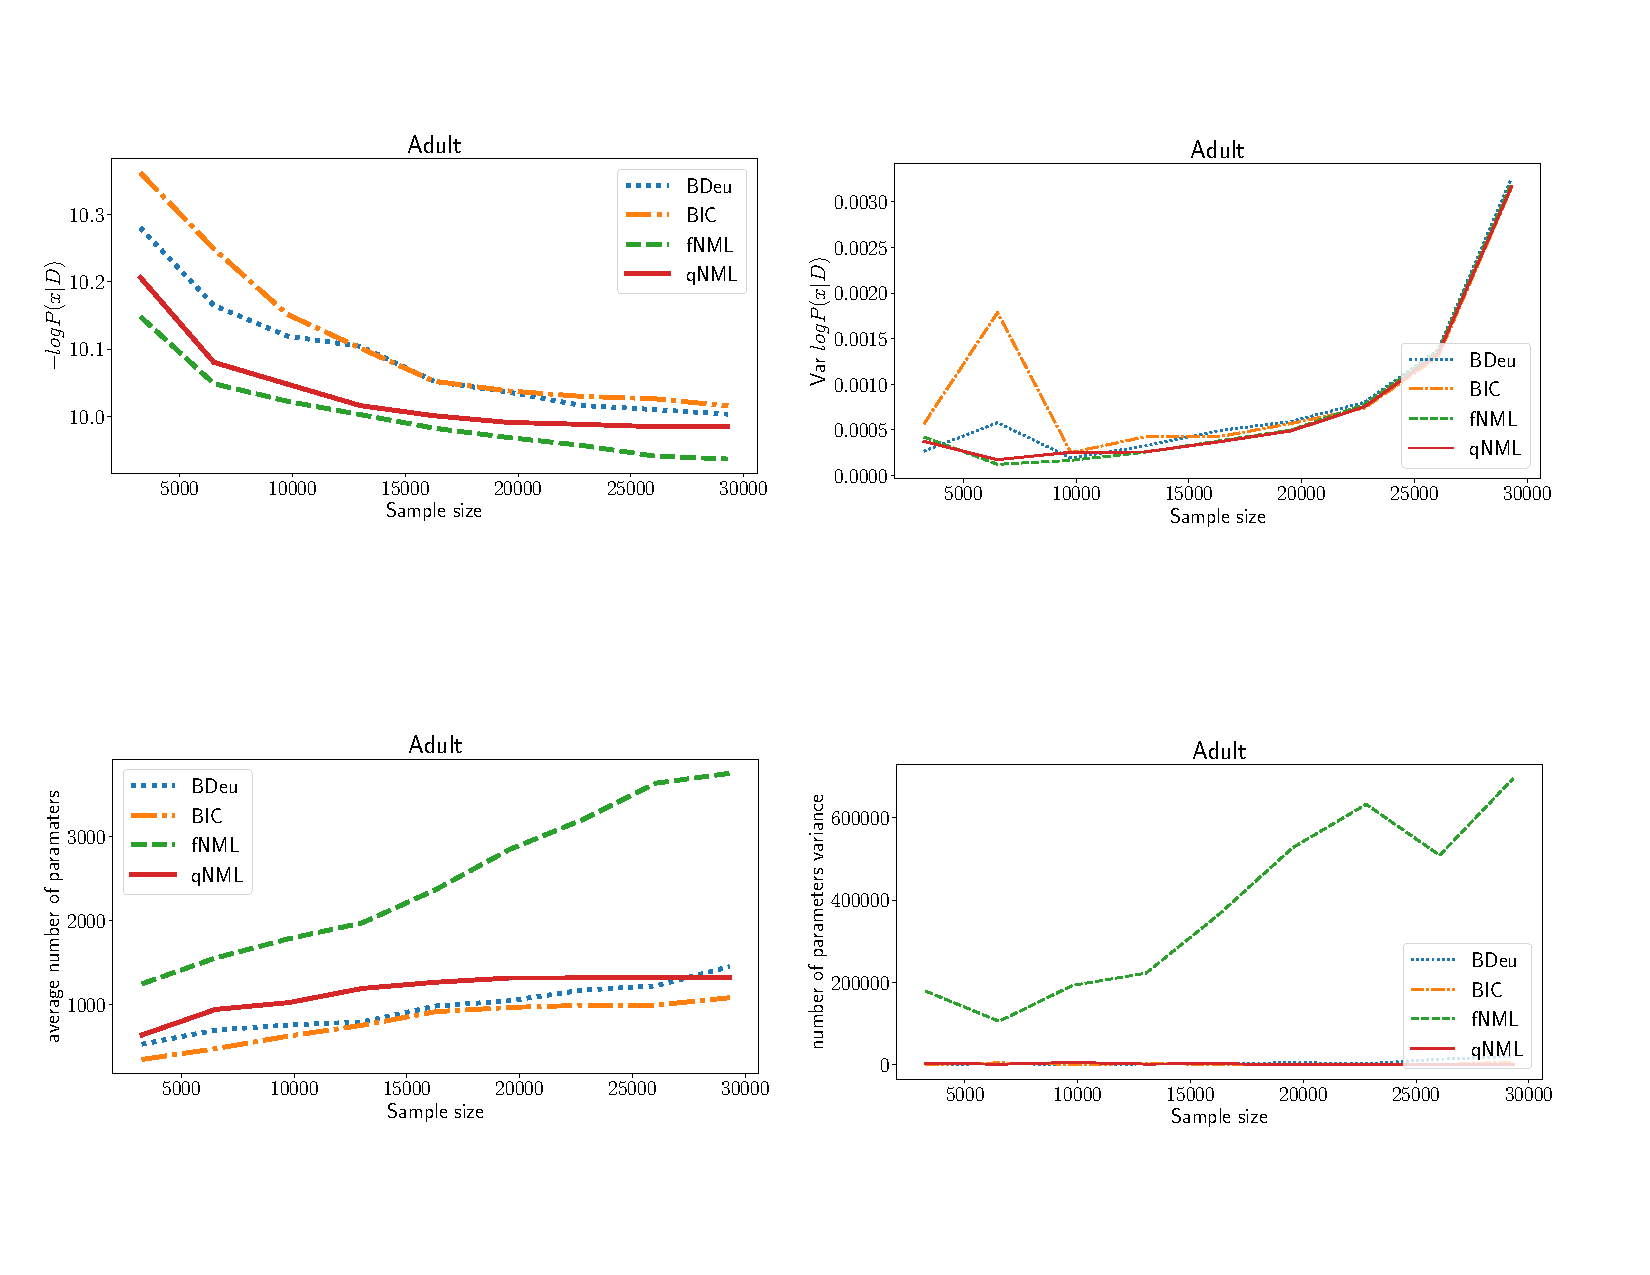
\includepdf[pages={1-20}]{all_qNML_images4.pdf}


\bibliographystyle{apalike}
\bibliography{cosco}
\end{document}
